\documentclass{article}

\usepackage{graphicx}
\usepackage{tikz}
\usepackage{tikzsymbols}
\usetikzlibrary{calc,patterns,shapes.geometric}
\pagestyle{empty}
\usepackage[margin=0pt]{geometry}
\geometry{papersize={14in,12in}}

\def\centerarc[#1](#2)(#3:#4:#5){\draw[#1] ($(#2)+({#5*cos(#3)},{#5*sin(#3)})$) arc (#3:#4:#5);}

\begin{document}
	\begin{figure}
		\centering
		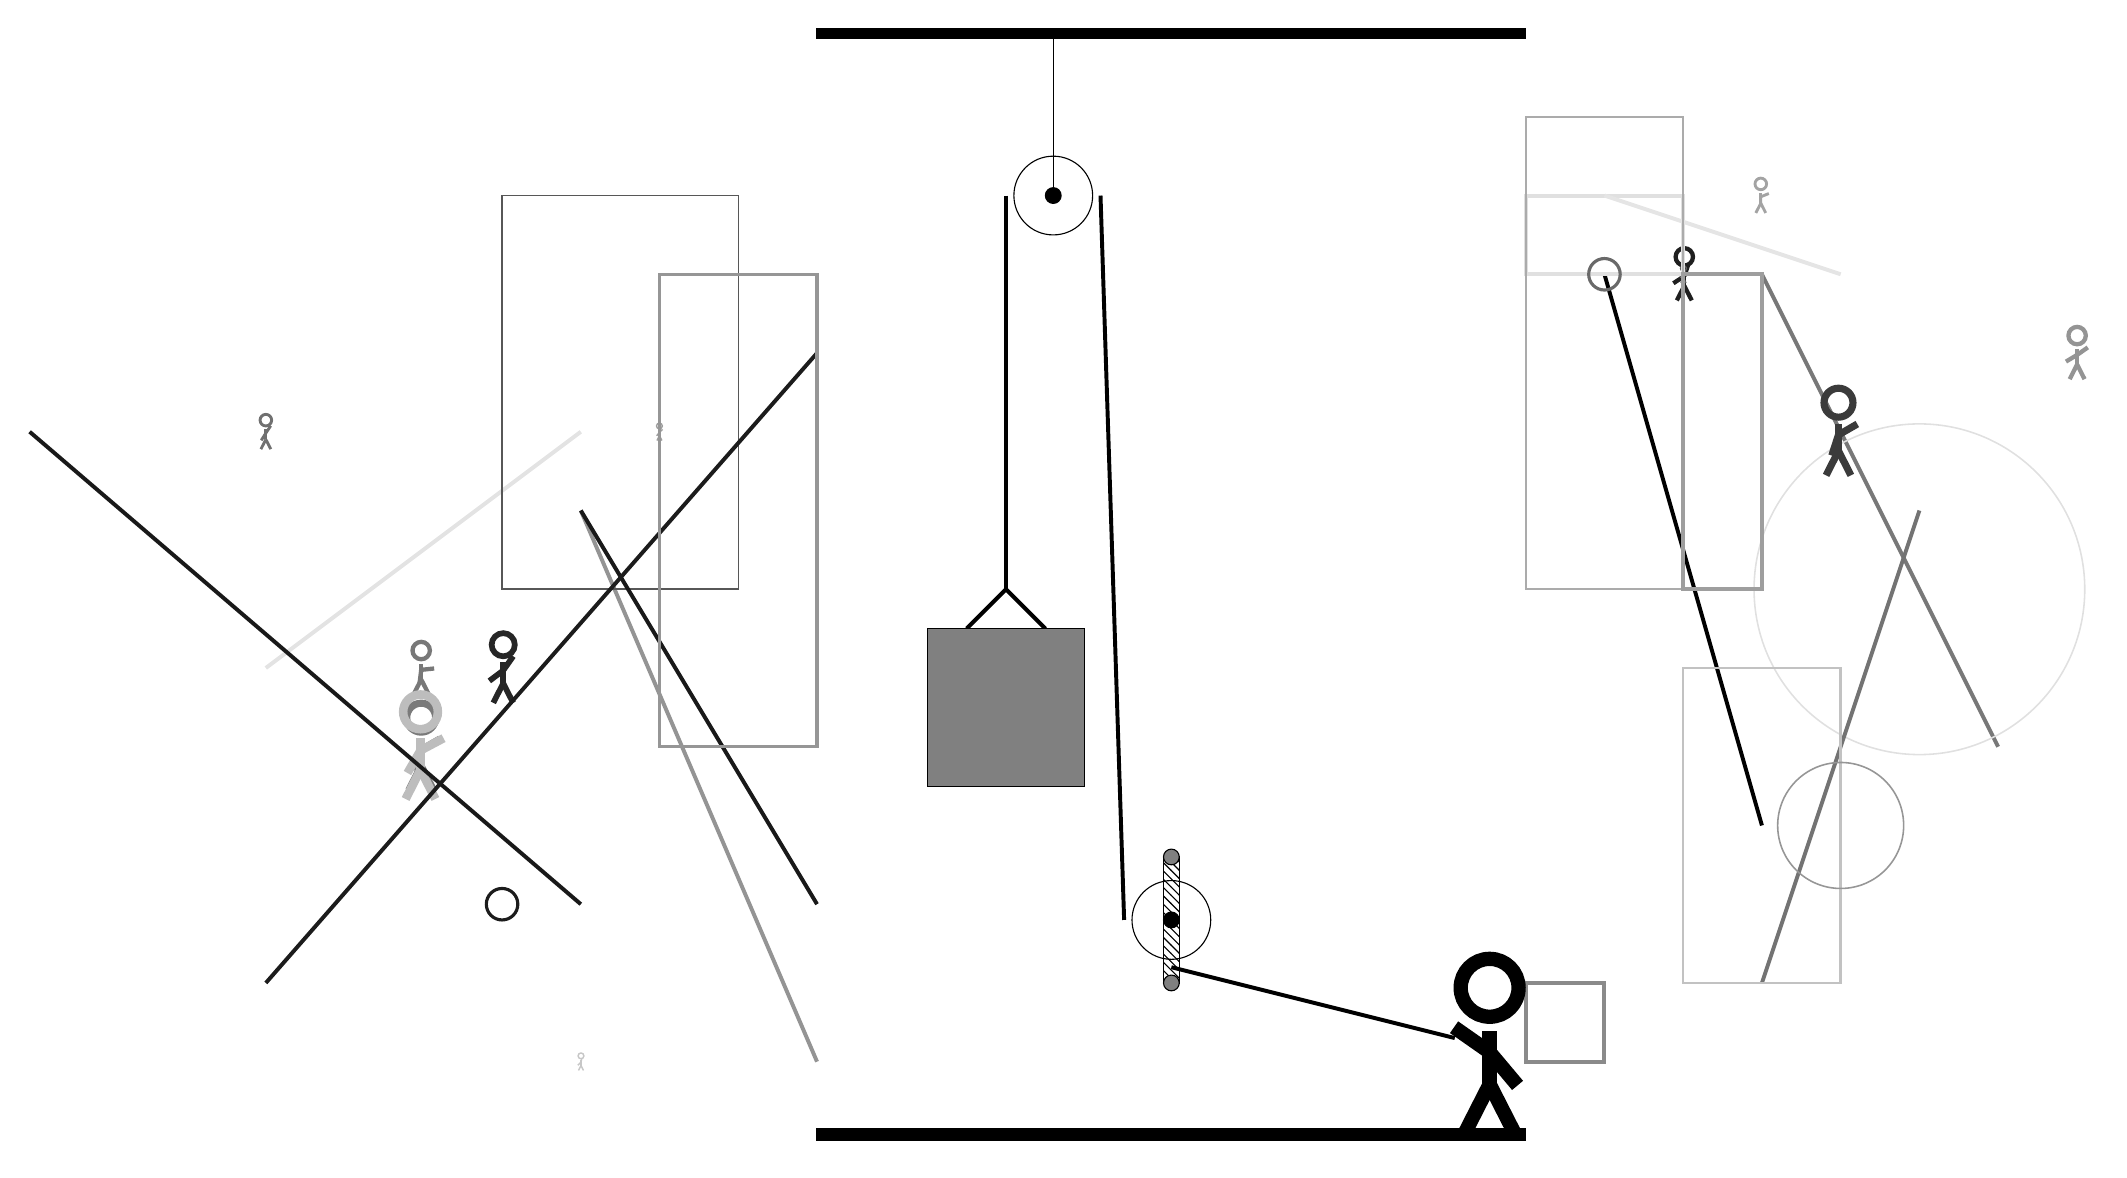
\begin{tikzpicture}
			%%%%% START %%%%%
			
			\draw[fill=black] (-2, 14) rectangle (7, 14.125);
			
			\draw (1, 12) circle (0.5);
			\draw[fill=black] (1, 12) circle (0.1);
			\draw (1, 14) -- (1, 12);
			
			\draw[fill=white](2.5, 2.8) circle (0.5);
			\draw[fill=black] (2.5, 2.8) circle (0.1);
			\draw[pattern=north west lines, pattern color=black] (2.4, 3.6) rectangle (2.6, 2.0);
			\draw[fill=black!50] (2.5, 3.6) circle (0.1);
			\draw[fill=black!50] (2.5, 2.0) circle (0.1);
			
			\node[line width=0.3mm, color=black!42] at (14, 10) {\Strichmaxerl[3][31][35]};
			
			\draw[line width=0.5mm, color=black!53](10, 11) -- (13, 5);
			\draw[line width=0.5mm, color=black!11](-5, 9) -- (-9, 6);
			\draw[line width=0.5mm, color=black!42](-2, 1) -- (-5, 8);
			\node[line width=0.3mm, color=black!52] at (-7, 5) {\Strichmaxerl[5][72][30]};
			\node[line width=0.3mm, color=black!88] at (9, 11) {\Strichmaxerl[3][33][71]};
			\draw [line width=0.2mm, color=black!12](12, 7) circle (2.1);
			
			\node[line width=0.2mm, color=black!36] at (10, 12) {\Strichmaxerl[2][89][22]};
			\draw[line width=0.5mm, color=black!100](8, 11) -- (10, 4);
			\node[line width=0.6mm, color=black!63] at (9, 11) {\Strichmaxerl[1][36][63]};
			\draw[line width=0.5mm, color=black!55](12, 8) -- (10, 2);
			
			\node[line width=0.6mm, color=black!85] at (-6, 6) {\Strichmaxerl[4][37][55]};
			\node[line width=0.6mm, color=black!53] at (-7, 6) {\Strichmaxerl[3][83][6]};
			\node[line width=0.4mm, color=black!56] at (-9, 9) {\Strichmaxerl[2][58][56]};
			\draw [line width=0.4mm, color=black!89](-6, 3) circle (0.2);
			\node[line width=0.7mm, color=black!26] at (-7, 5) {\Strichmaxerl[6][60][28]};
			
			\draw[line width=0.3mm, color=black!24] (9, 6) rectangle (11, 2);
			\node[line width=0.7mm, color=black!77] at (11, 9) {\Strichmaxerl[5][72][30]};
			\node[line width=0.6mm, color=black!22] at (-5, 1) {\Strichmaxerl[1][42][79]};
			
			\draw [line width=0.2mm, color=black!41](11, 4) circle (0.8);
			\draw[line width=0.5mm, color=black!12] (7, 11) rectangle (9, 12);
			\draw[line width=0.5mm, color=black!10](8, 12) -- (11, 11);
			\draw[line width=0.2mm, color=black!33] (7, 13) rectangle (9, 7);
			\draw[line width=0.5mm, color=black!38] (9, 7) rectangle (10, 11);
			\draw[line width=0.5mm, color=black!90](-5, 3) -- (-12, 9);
			\draw[line width=0.2mm, color=black!66] (-3, 7) rectangle (-6, 12);
			\draw[line width=0.5mm, color=black!90](-2, 3) -- (-5, 8);
			\draw[line width=0.5mm, color=black!46] (8, 1) rectangle (7, 2);
			\node[line width=0.6mm, color=black!38] at (-4, 9) {\Strichmaxerl[1][51][43]};
			\draw[line width=0.5mm, color=black!89](-2, 10) -- (-9, 2);
			\draw [line width=0.4mm, color=black!59](8, 11) circle (0.2);
			
			\draw[line width=0.5mm, color=black!89](11, 2) -- (11, 2);
			\draw[line width=0.4mm, color=black!41] (-2, 11) rectangle (-4, 5);
			
			\draw[line width=0.5mm] (-0.1, 6.5) -- (0.4, 7.0) -- (0.9, 6.5);
			\draw[fill=black!50] (-0.6, 6.5) rectangle (1.4, 4.5);
			
			\draw[line width=0.5mm] (0.4, 12) -- (0.4, 7.0);
			\centerarc[line width=0.5mm](1, 12)(0:180:0.6);
			\draw[line width=0.5mm](1.6, 12) -- (1.9, 2.8);
			\centerarc[line width=0.5mm](2.5, 2.8)(180:270:0.6);
			\draw[line width=0.5mm](2.5, 2.2) -- (6.1, 1.3);
			
			\node at (6.5, 1.2) {\Strichmaxerl[10][-35][-50]};
			
			\draw[fill=black] (-2, 0) rectangle (7, 0.15);
			
			%%%%% END %%%%%
		\end{tikzpicture}
	\end{figure}	
\end{document}